\documentclass[openbib]{article}

\usepackage{color}
\usepackage{ctex}
\usepackage{float}
\usepackage{mathtools}
\usepackage{amsmath}
\usepackage{graphicx}
% Copyright 20120 Liutao Tian, MIT License
% https://github.com/andy123t/code-latex-style/

\usepackage{listings,color}

% Matlab highlight color settings
%\definecolor{mBasic}{RGB}{248,248,242}       % default
\definecolor{mKeyword}{RGB}{0,0,255}          % bule
\definecolor{mString}{RGB}{160,32,240}        % purple
\definecolor{mComment}{RGB}{34,139,34}        % green
\definecolor{mBackground}{RGB}{245,245,245}   % lightgrey
\definecolor{mNumber}{RGB}{134,145,148}       % gray

\definecolor{Numberbg}{RGB}{237,240,241}     % lightgrey

% Python highlight color settings
%\definecolor{pBasic}{RGB}{248, 248, 242}     % default
\definecolor{pKeyword}{RGB}{228,0,128}        % magenta
\definecolor{pString}{RGB}{148,0,209}         % purple
\definecolor{pComment}{RGB}{117,113,94}       % gray
\definecolor{pIdentifier}{RGB}{166, 226, 46}  %
\definecolor{pBackground}{RGB}{245,245,245}   % lightgrey
\definecolor{pNumber}{RGB}{134,145,148}       % gray

\lstnewenvironment{Python}[1]{
	\lstset{language=python,               % choose the language of the code
		xleftmargin=30pt,
		xrightmargin=10pt,
		frame=l,
		framesep=15pt,%framerule=0pt,  % sets the frame style
		%frame=shadowbox,rulesepcolor=\color{red!20!green!20!blue!20},
		%basicstyle=\small\ttfamily,          % sets font style for the code
		basicstyle=\footnotesize\fontspec{Consolas},
		keywordstyle=\color{pKeyword},       % sets color for keywords
		stringstyle=\color{pString},         % sets color for strings
		commentstyle=\color{pComment},       % sets color for comments
		backgroundcolor=\color{pBackground}, % choose the background color
		title=#1,                            %\lstname show the filename of files
		emph={format_string,eff_ana_bf,permute,eff_ana_btr},
		emphstyle=\color{pIdentifier}
		showspaces=false,                    % show spaces adding particular underscores
		showstringspaces=false,              % underline spaces within strings
		showtabs=false,                      % show tabs within strings adding particular underscores
		tabsize=4,                           % sets default tabsize to 2 spaces
		captionpos=t,                        % sets the caption-position to bottom
		breaklines=true,                     % sets automatic line breaking
		framexleftmargin=5pt,
		fillcolor=\color{Numberbg},
		rulecolor=\color{Numberbg},
		numberstyle=\tiny\color{pNumber},
		numbersep=9pt,                      % how far the line-numbers are from the code
		numbers=left,                        % where to put the line-numbers
		stepnumber=1,                        % the step between two line-numbers.
}}{}

\lstnewenvironment{Python1}[1]{
\lstset{language=python,               % choose the language of the code
  xleftmargin=30pt,
  xrightmargin=10pt,
  frame=l,
  framesep=15pt,%framerule=0pt,  % sets the frame style
  %frame=shadowbox,rulesepcolor=\color{red!20!green!20!blue!20},
  %basicstyle=\small\ttfamily,          % sets font style for the code
  basicstyle=\footnotesize\fontspec{Consolas},
  keywordstyle=\color{pKeyword},       % sets color for keywords
  stringstyle=\color{pString},         % sets color for strings
  commentstyle=\color{pComment},       % sets color for comments
  backgroundcolor=\color{pBackground}, % choose the background color
  title=#1,                            %\lstname show the filename of files
  emph={format_string,eff_ana_bf,permute,eff_ana_btr},
  emphstyle=\color{pIdentifier}
  showspaces=false,                    % show spaces adding particular underscores
  showstringspaces=false,              % underline spaces within strings
  showtabs=false,                      % show tabs within strings adding particular underscores
  tabsize=4,                           % sets default tabsize to 2 spaces
  captionpos=t,                        % sets the caption-position to bottom
  breaklines=true,                     % sets automatic line breaking
  framexleftmargin=5pt,
  fillcolor=\color{Numberbg},
  rulecolor=\color{Numberbg},
  numberstyle=\tiny\color{pNumber},
  numbersep=9pt,                      % how far the line-numbers are from the code
  numbers=left,                        % where to put the line-numbers
  stepnumber=1,                        % the step between two line-numbers.
}}{}



\usepackage{fontspec}
\graphicspath{{figures/}}
\renewcommand{\contentsname}{\centerline{目录}}

\begin{document}
	\title{循环神经网络}
	
	%	https://www.paddlepaddle.org.cn/	数据集https://www.kaggle.com   论文集https://arxiv.org/
	%	CVPR,ECCV,ICCV	
	
	\maketitle
	
	\newpage
	\tableofcontents
	\newpage
\section{循环神经网络简介}
多层感知机和卷积神经网络这样的前馈神经网络,理论上可以完成从确定形式的输入到确定的输出的任何映射。但是前馈网络的输入都是相互独立的,实际的任务中经常会出现模型的输入不仅与当前时刻的输入有关,还与过去的某个状态有关。

一般地,前馈神经网络对于序列数据的处理都存在一定的困难。原因在于序列数据的长度通常不固定,并且元素的顺序排列由多种。对于序列化数据,考虑到序列的长度,顺序等因素,我们必须在模型的不同部分使用相同的参数。因此,参数共享作为循环神经网络的一大特点,为循环神经网络带来了强大的泛化能力(针对序列长度和顺序的泛化)。循环神经网络的短期记忆能力:隐藏层神经元不仅能够接受其他神经元的信息,还可以接受上一时刻自身的信息,从而形成一个小环路结构。循环神经网络(Recurrent Neural Network,RNN)挖掘数据中的时序信息以及语义信息的深度表达能力被充分利用,用于处理和预测序列数据,广泛应用于语音识别,手写体识别。
\subsection{循环神经网络的结构与计算能力}
循环神经网络是一个在时间上传递的神经网络,网络的深度就是时间的长度。该神经网络是专门用来处理时间序列问题的,能够提取时间序列的信息。

给定一个输入序列$sx_{1:T} = (x_1,x_2,...,x_T)$,循环神经网络主要通过带反馈的隐藏层单元来建模序列信息。$$f_i=f(h_{t-1},x_i)$$
其中,$h_0$=0代表初始隐藏层信息,f()为非线性激活函数,也可以是一个前馈神经网络。

对于简单循环网络计算图,输入层到隐藏层的参数为权重矩阵\textbf{U},隐藏层到输出层打参数为权重\textbf{V},隐藏层到隐藏层的反馈连接参数为权重矩阵\textbf{W},则该循环神经网络的前向传播公式为:
$$a_t = b+\textbf{W}h_{t-1}+\textbf{U}x_t$$
$$h_t = tanh(a_t)$$
$$o_t = c + \textbf{V}h_t$$
该循环神经网络将一个输入序列映射为相同长度的输出序列。对于分类任务:将输出层的神经元分别通过softmax分类层进行分类;对于回归任务:直接将输出层神经元的信息作为需要使用的回归值。

如图,循环体中的神经网络的输入有两部分:一个是上个时刻的状态,另一个是当前时刻的输入样本。它由输入层,隐藏层,输出层组成。
\begin{figure}[htbp]
	\centering
	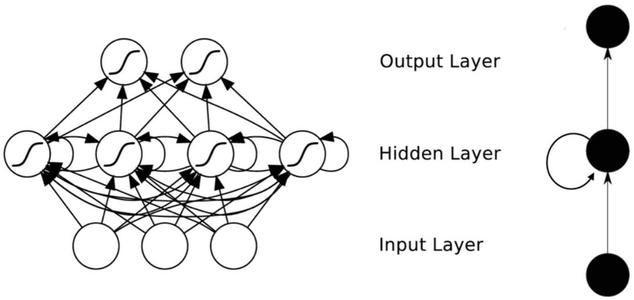
\includegraphics[scale=0.5]{循环神经网络结构模型.jpg}
\end{figure}

循环神经网络的隐藏层相互连接,即一个序列当前的输出与前面的输出也有关。循环神经网络会对于每一个时刻的输入结合当前模型的状态给出一个输出。RNN对序列的每个元素执行同样的操作,其输出依赖于前次计算的结果。RNN引入了定向循环,能够处理那些输入之间前后关联的问题。RNN拥有捕获已计算节点信息的记忆能力。

\begin{figure}[htbp]
	\centering
	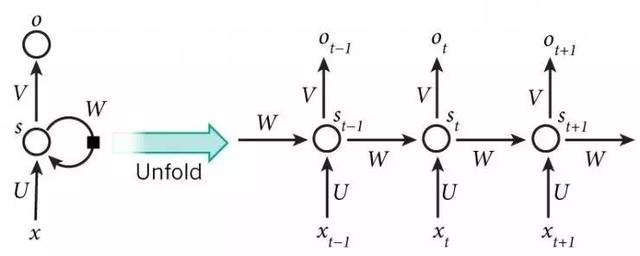
\includegraphics[scale=0.5]{循环神经网络展开图.jpg}
\end{figure}

x是输入层的值,s是隐藏层的值,U是输入层和隐藏层的权重矩阵,o表示输出层的值,V是隐藏层到输出层的权重矩阵。循环神经网络的隐藏层的值s不仅仅取决于当前这次的输入x,还取决于上一次隐藏层的值s。权重矩阵W就是隐藏层上一次的值作为这一次的输入权重。对于一个序列数据,可以将这个序列上不同时刻的数据依次传入循环神经网络的输入层,而输出可以是对序列中下一时刻的预测,也可以是对当前时刻信息的处理结果。

循环神经网络中由于输入时叠加了之前的信号,所以反向传导时不同于传统的神经网络,对于时刻t的输入层,其残差不仅来自输出,还来自隐藏层。

通过反向传递算法,利用输出层的误差,求解各个权重的梯度,然后利用梯度下降法更新各个权重。展开图中信息流向时确定的,没有环流,循环神经系统是时间维度上的深度模型,可以对序列内容建模。但需要训练的参数较多,容易出现梯度消失或梯度爆炸的问题,不具有特征学习能力。

根据通用近似定理(Universal Approximation Theorem)前馈神经网络可以拟合任何的连续函数。一个有足够数量的sigmoid型隐藏单元的完全连接的循环神经网络,可以以任意精度拟合任意一个非线性动力系统:
$$s_t = g(s_{t-1},x_t)$$
$$y_t = o(s_t)$$
其中,$s_t$表示当前时刻的系统状态,$x_t$表示当时时刻对系统的输入,g()表示可测的状态转移函数(非线性函数),o()表示系统输出的连续函数。

一个使用sigmoid型隐藏单元的完全连接的循环神经网络还是图灵完备(Turing Completeness)的,即可以近似解决所有可计算问题。
\subsection{参数学习}
对于分类任务,该模型的损失函数为分类交叉熵损失;对于回归任务,该模型的损失函数为平方损失。

计算该损失函数计算模型中各个参数的梯度是一个计算成本很高的操作,循环神经网络的反向传播从右到左进行,由于是按序的前向传播,使得复杂度无法通过并行来降低。

\begin{center}
	1.通过时间反向传播(Back Propagation Through Time,BPTT)
\end{center}
通过计算图沿时间方向的展开,可以沿着前向传播的反方向对计算图中的节点依次求梯度,然后再让模型的参数通过梯度下降的方向来改进,从而降低损失函数,即利用该损失函数展开计算图的反向传播算法。就是简单的将传统的BP算法推广到循环神经网络的展开计算图上。计算图的节点包括参数U,V,W,b和c以及每个时间步节点的信息$x_t$,$h_t$,$o_t$和$L_t$

在计算模型的输出序列中所有神经元的预测值$o_t$和目标值$y_t$的平方损失,再将时间序列中的T个损失相加得到总损失函数:
$$L=\sum_{t=1}^{T}\frac{1}{2}(o_t-y_t)^T(o_t-y_t)$$
首先计算输出层神经元的导数:
$$\frac{\partial L}{\partial L_t}=1$$
$$\frac{\partial L}{\partial o_t}=\frac{\partial L}{\partial L_t}\frac{\partial L_t}{\partial o_t}=(o_t - y_t)^T$$
计算隐藏层节点的导数时,要分两种情况考虑:

先考虑最后一个时间步(第T个时间步)隐藏层的导数:
$$\frac{\partial L}{\partial h_T}= \frac{\partial L}{\partial o_T}V$$

再考虑前T-1个时间步中隐藏层的导数时,需要注意每个隐藏层神经元的导数不仅与输出层有关,还与下个时间步的隐藏层有关,前T-1个隐藏层的导数为:
$$\frac{\partial L}{\partial h_t}=\frac{\partial L_t}{\partial h_t}+\frac{\partial L}{\partial h_{t+1}}\frac{\partial h_{t+1}}{\partial h_t}= \frac{\partial L}{\partial o_t}V+\frac{\partial L}{\partial h_{t+1}}diag(1-h_{t+1}^2)W$$
其中,$h_{t+1}^2$表示隐藏层向量$h_{t+1}$中每个元素的平方组成的新向量;$diag(1-h_{t+1}^2)$表示对角线元素为$1-h_{t+1}^2$的对角矩阵,这是t+1时刻的隐藏层单元关于$a_{t+1}$的双曲正切函数的雅克比矩阵。

故能够得到损失函数关于模型各参数节点的梯度。
$$\frac{\partial L]}{\partial c}=\sum_{t=1}^{T}\frac{\partial L}{\partial o_t}\frac{\partial o_t}{\partial c}=\sum_{t=1}^{T}\frac{\partial L}{\partial o_t}$$

$$\frac{\partial L}{\partial b}=\sum_{t=1}^{T}\frac{\partial L}{\partial h_t}\frac{\partial h_t}{\partial b}=\sum_{t=1}^{T}\frac{\partial L}{\partial h_t}diag(1-h_t^2)$$

以下推导涉及向量对矩阵的导数,将向量中的元素依次提取成标量对矩阵的导数。然后再将求和的结果归纳成向量乘积的形式。
$$\frac{\partial L}{\partial V}=\sum_{t=1}^{T}\sum_{i=1}^{len(o)}\frac{\partial L}{\partial o_{t+1}}\frac{\partial o_{t+1}}{\partial V}=\sum_{t=1}^{T}h_t\frac{\partial L}{\partial o_t}$$
其中,len(o)表示输出层向量的维度,$o_{t,i}$表示第t步输出层向量第i个元素的值。
$$\frac{\partial L}{\partial W}=\sum_{t=2}^{T}\sum_{i=1}^{len(h)}\frac{\partial L}{\partial h_{t,i}}\frac{\partial h_{t,i}}{\partial W}=\sum_{t=2}^{T}h_{t-1}\frac{\partial L}{\partial h_t}diag(1-h_i^2)$$
其中,len(h)表示输出层向量的维度,$h_{t,i}$表示第t步输出层向量第i个元素的值。
$$\frac{\partial L}{\partial U}=\sum_{t=1}^{T}\sum_{i=1}^{len(h)}\frac{\partial L}{\partial h_{t,i}}\frac{\partial h_{t,i}}{\partial U}=\sum_{t=1}^{T}x_i\frac{\partial L}{\partial h_t}diag(1-h_t^2)$$

\begin{center}
	2.实时循环学习(Real-Time Recurrent Learning,RTRL)
\end{center}
循环神经网络的参数是共享的,前向传播时就可以计算出相应的中间梯度值而丢弃之前的状态;最后根据这些中间梯度值通过链式求导法则直接得到对应参数的导数。推导公式使用分子布局方式。

首先,根据简单循环网络的前向传播公式,得到每一时间步应当保存下来的梯度值:
$$\frac{\partial h_t}{\partial W_{ij}}=\frac{\partial h_t}{\partial a_t}(\frac{\partial a_t}{\partial W_{ij}}+\frac{\partial a_t}{\partial h_{t-1}}\frac{\partial h_{t-1}}{\partial W_{ij}})=diag(1-h_t^2)(p_i(h_{t-1,j})+W\frac{\partial h_{t-1}}{\partial W_{ij}})$$
其中,$W_{ij}$表示参数矩阵W的第i行,第j列的值,$h_{t-1,j}$表示第t-1步隐藏层向量第j个元素的值,$p_i(h_{t-1,j})$表示只有第i个元素值为$h_{t-1,j}$,其余值都为0的向量。
$$\frac{\partial h_t}{\partial U_{ij}}=\frac{\partial h_t}{\partial a_t}(\frac{\partial a_t}{\partial U_{ij}}+\frac{\partial a_t}{\partial h_{t-1}}\frac{\partial h_{t-1}}{\partial U_{ij}})=diag(1-h_t^2)(p_i(x_{t,j})+W\frac{\partial h_{t-1}}{\partial U_{ij}})$$
其中,$U_{ij}$表示参数矩阵U的第i行,第j列的值,$x_{t,j}$表示第t步隐藏层向量第j个元素的值,$p_i(x_{t,j})$表示只有第i个元素值为$x_{t,j}$,其余值都为0的向量。
$$\frac{\partial h_t}{\partial b}=\frac{\partial h_t}{\partial a_t}(\frac{\partial a_t}{\partial b}+\frac{\partial a_t}{\partial h_{t-1}}\frac{\partial h_{t-1}}{\partial b})=diag(1-h_t^2)(I+W\frac{\partial h_{t-1}}{\partial b})$$
然后,当第t个时间步存在输出时,我们就可以通过链式求导法则得到此刻的损失函数对各个参数的导数值。
$$\frac{\partial L_t}{\partial c}=\frac{\partial L_t}{\partial o_t}\frac{\partial o_t}{\partial c}=\frac{\partial L_t}{\partial o_t}$$
$$\frac{\partial L_t}{\partial V}=h_t\frac{\partial L_t}{\partial o_t}$$
$$\frac{\partial L_t}{\partial W_{ij}}=\frac{\partial L_t}{\partial o_t}\frac{\partial o_t}{\partial h_t}\frac{\partial h_t}{\partial W_{ij}}=\frac{\partial L_i}{\partial o_t}V\frac{\partial h_t}{\partial W_{ij}}$$
$$\frac{\partial L_t}{\partial U_{ij}}=\frac{\partial L_t}{\partial o_t}\frac{\partial o_t}{\partial h_t}\frac{\partial h_t}{\partial U_{ij}}=\frac{\partial L_i}{\partial o_t}V\frac{\partial h_t}{\partial U_{ij}}$$
$$\frac{\partial L_t}{\partial b}=\frac{\partial L_t}{\partial o_t}\frac{\partial o_t}{\partial h_t}\frac{\partial h_t}{\partial b}=\frac{\partial L_i}{\partial o_t}V\frac{\partial h_t}{\partial b}$$

最后,如果网络有多个输出和多个损失函数,需要将这些损失函数的梯度相加,才能得到最终的损失函数对模型中各个参数的导数。以上为分子布局,需要变为分母布局才能进行梯度下降优化。

BPTT算法比RTRL算法计算量更小,因为一般模型的输入向量的维度要远远大于输出向量的维度。
RTRL算法在使用完上一时间的偏导数后就可以删去,更节约空间,另外不需要梯度反转,梯度的计算可以在前向传播中完成,更适合在线学习或无限序列的训练任务。
\subsection{不同的RNN}
\begin{center}
	1.Simple RNN(SRN)
\end{center}

它是一个三层网络,并且在隐藏层增加了上下文单元,上下文单元节点于隐藏层中的节点的连接是固定的,并且权值也是固定的。

在每一步中,使用标准的前向反馈进行传播,然后使用学习算法进行学习。保存上文:上下文每个节点保存其连接的隐藏层节点的每上一步的输出,并作用于当前步对应的隐藏层节点的状态,即隐藏层的输入由输入层的输出与上一步自己的状态所决定。能够对序列数据进行预测。
\begin{Python}{SRN}
	import numpy as np
	
	
	class RNN:
	
	def __init__(self, in_shape, unit, out_shape):
	'''
	:param in_shape: 输入x向量的长度
	:param unit: 隐层大小
	:param out_shape: 输出y向量的长度
	'''
	self.U = np.random.random(size=(in_shape, unit))
	self.W = np.random.random(size=(unit, unit))
	self.V = np.random.random(size=(unit, out_shape))
	
	self.in_shape = in_shape
	self.unit = unit
	self.out_shape = out_shape
	
	self.start_h = np.random.random(size=(self.unit,))  # 初始隐层状态
	
	@staticmethod
	def tanh(x):
	return (np.exp(x)-np.exp(-x))/(np.exp(x)+np.exp(-x))
	
	@staticmethod
	def tanh_der(y):
	return 1 - y*y
	
	@staticmethod
	def softmax(x):
	tmp = np.exp(x)
	return tmp/sum(tmp)
	
	@staticmethod
	def softmax_der(y, y_):
	j = np.argmax(y_)
	tmp = y[j]
	y = -y[j]*y
	y[j] = tmp*(1-tmp)
	return y
	
	@staticmethod
	def cross_entropy(y, y_):
	'''
	交叉熵
	:param y:预测值
	:param y_: 真值
	:return:
	'''
	return sum(-np.log(y)*y_)
	
	@staticmethod
	def cross_entropy_der(y, y_):
	j = np.argmax(y_)
	return -1/y[j]
	
	def inference(self, x, h_1):
	'''
	前向传播
	:param x: 输入向量
	:param h_1: 上一隐层
	:return:
	'''
	h = self.tanh(np.dot(x, self.U) + np.dot(h_1, self.W))
	y = self.softmax(np.dot(h, self.V))
	return h, y
	
	def train(self, x_data, y_data, alpha=0.1, steps=100):
	'''
	训练RNN
	:param x_data: 输入样本
	:param y_data: 标签
	:param alpha: 学习率
	:param steps: 迭代伦次
	:return:
	'''
	for step in range(steps):  # 迭代伦次
	print("step:", step+1)
	for xs, ys in zip(x_data,y_data):  # 每个样本
	h_list = []
	h = self.start_h  # 初始化初始隐层状态
	h_list.append(h)
	y_list = []
	losses = []
	for x, y_ in zip(xs, ys):  # 前向传播
	h, y = self.inference(x, h)
	loss = self.cross_entropy(y=y, y_=y_)
	h_list.append(h)
	y_list.append(y)
	losses.append(loss)
	print("loss:", np.mean(losses))
	V_update = np.zeros(shape=self.V.shape)
	U_update = np.zeros(shape=self.U.shape)
	W_update = np.zeros(shape=self.W.shape)
	next_layer1_delta = np.zeros(shape=(self.unit,))
	
	for i in range(len(xs))[::-1]:  # 反向传播
	layer2_delta = -self.cross_entropy_der(y_list[i], ys[i])*self.softmax_der(y_list[i], ys[i])  # 输出层误差
	# 当前隐层梯度 = 下一隐层梯度 * 下一隐层权重 + 输出层梯度 * 输出层权重
	layer1_delta = self.tanh_der(h_list[i+1])*(np.dot(layer2_delta, self.V.T) + np.dot(next_layer1_delta, self.W.T))
	
	V_update += np.dot(np.atleast_2d(h_list[i+1]).T, np.atleast_2d(layer2_delta))  # V增量
	W_update += np.dot(np.atleast_2d(h_list[i]).T,  np.atleast_2d(layer1_delta))  # W增量
	U_update += np.dot(np.atleast_2d(xs[i]).T,  np.atleast_2d(layer1_delta))  # U增量
	
	next_layer1_delta = layer1_delta  # 更新下一隐层的梯度等于当前隐层的梯度
	self.W += W_update * alpha
	self.V += V_update * alpha
	self.U += U_update * alpha
	# print(self.W,self.V,self.U)
	
	def predict(self, xs, return_sequence=False):
	'''
	RNN预测
	:param xs: 单个样本
	:param return_sequence: 是否返回整个输出序列
	:return:
	'''
	
	y_list = []
	h_list = []
	h = self.start_h
	for x in xs:
	h, y = self.inference(x,h)
	y_list.append(y)
	h_list.append(h)
	if return_sequence:
	return h_list, y_list
	else:
	return h_list[-1], y_list[-1]
	
	class RNNTest:
	
	def __init__(self, hidden_num, all_chars):
	'''
	创建一个rnn
	:param hidden_num: 隐层数目
	:param all_chars: 所有字符集
	'''
	self.all_chars = all_chars
	self.len = len(all_chars)
	self.rnn = RNN(self.len, hidden_num, self.len)
	
	def str2onehots(self, string):
	'''
	字符串转独热码
	:param string:
	:return:
	'''
	one_hots = []
	for char in string:
	one_hot = np.zeros((self.len,),dtype=np.int)
	one_hot[self.all_chars.index(char)] = 1
	one_hots.append(one_hot)
	return one_hots
	
	def vector2char(self, vector):
	'''
	预测向量转字符
	:param vector:
	:return:
	'''
	return self.all_chars[int(np.argmax(vector))]
	
	def run(self, x_data, y_data, alpha=0.1, steps=500):
	
	x_data_onehot = [self.str2onehots(xs) for xs in x_data]
	y_data_onehot = [self.str2onehots(ys) for ys in y_data]
	self.rnn.train(x_data_onehot, y_data_onehot, alpha=alpha, steps=steps) # 训练
	vector_f = self.rnn.predict(self.str2onehots("c"), False)[1] # 预测f下一个字母
	vector_ab = self.rnn.predict(self.str2onehots("fg"), False)[1] # 预测ab的下一个字母
	print("c.next=",self.vector2char(vector_f))
	print("fg.next=",self.vector2char(vector_ab))
	
	
	# 测试:下一个字母
	x_data = ["abc","bcd","cdef","fgh","a","bc","abcdef"]
	y_data = ["bcd","cde","defg","ghi","b","cd","bcdefg"]
	all_chars = "abcdefghi"
	
	rnn_test = RNNTest(10, all_chars)
	rnn_test.run(x_data,y_data)
	
\end{Python}

\begin{center}
	2.Bidrectional RNN
\end{center}

双向RNN是两个RNN上下叠加在一起组成的,当前的输出和之前的序列元素,以及之后的序列元素都是有关系的。比如:预测语句中缺失的词语就需要根据上下文来预测。输出是由两个RNN的隐藏层的状态决定的。

\begin{center}
	3.深层双向RNN
\end{center}

深层双向RNN和双向RNN类似,区别只是每一步/每个时间点设定为多层结构。

\begin{center}
	4.LSTM神经网络
\end{center}

Long Short Term网络,LSTM精确解决了RNN的长短记忆问题。在LSTM中,有一个“输入门”(input gate),一个“遗忘门”(forget gate),一个“输出门”(output gate)。
\begin{figure}[htbp]
	\centering
	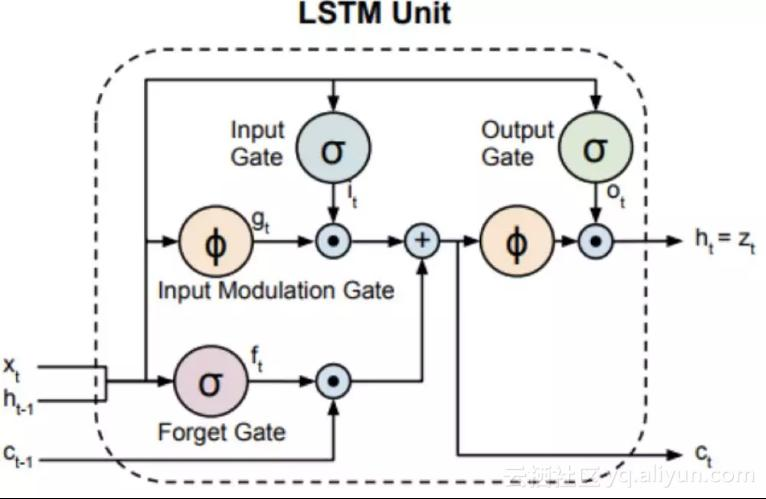
\includegraphics[scale=0.3]{LSTM神经网络结构图}
\end{figure}

输入门$i_t$:控制有多少信息可以流入记忆细胞。

遗忘门$f_t$:控制有多少上一时刻的记忆细胞中的信息可以积累到当前时刻的记忆细胞中。

输出门$o_t$:控制有多少当前时刻的记忆细胞中的信息可以流入当前隐藏状态$h_t$中

各个unit称为cell,它们可以结合前面的状态,当前的记忆与当前的输入。该网络结构在对长序列依赖问题中非常有效。LSTM神经元的输出除了与当前输入有关外,还与自身记忆有关。RNN的训练算法也是基于传统BP算法,并且增加了时间考量,称为BPTT(Back-propagation Through Time)算法。
\begin{figure}[htbp]
	\centering
	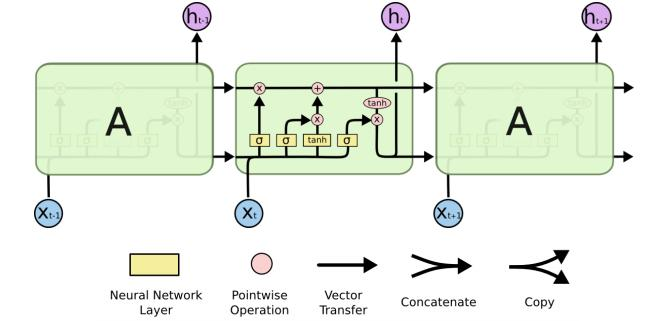
\includegraphics[scale=0.42]{LSTM内部结构}
\end{figure}

Neural NetWork Layer:表示一个神经网络层

Pointwise Operation:表示一种数学操作

Vector Transfer:表示每条线代表一个向量,从一个节点输出到另一个节点

Concatenate:表示两个向量的合并

Copy:表示复制一个向量变成相同的两个向量
\subsection{LSTM结构具体解析}
\begin{figure}[H]
	\centering
	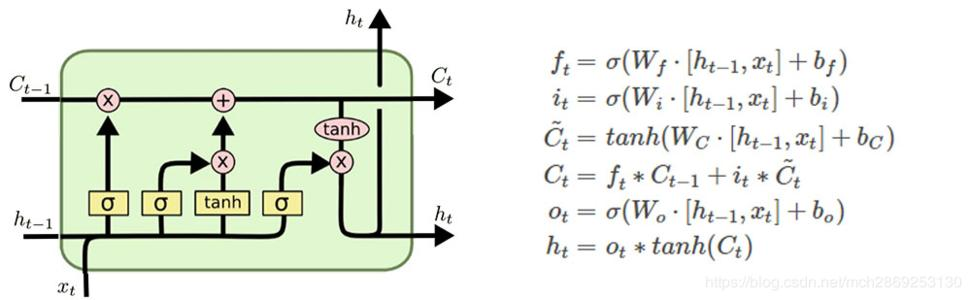
\includegraphics[scale=0.4]{LSTM}
\end{figure}
第一步:利用遗忘门层,决定从细胞状态中丢弃什么信息。读取$h_{t-1}$和$x_t$,输出一个在0到1之间的数值给每个在细胞状态$C_{t-1}$中的数字。由于Sigmoid输出结果为0和1,所以用1表示“完全保留”,0表示“完全舍弃”。
\begin{figure}[H]
	\centering
	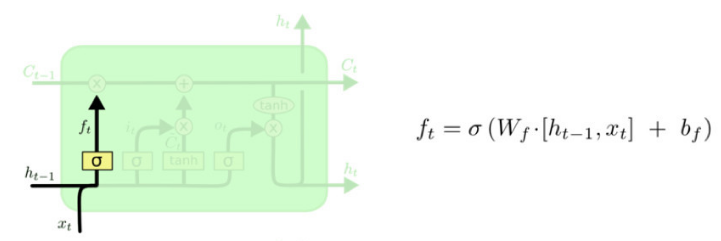
\includegraphics[scale=0.4]{衰减系数计算过程}
\end{figure}

第二步:更新信息。首先,Sigmoid层为“输入门层”,决定什么值将要更新。然后tanh层创建一个新的候选值向量。
\begin{figure}[H]
	\centering
	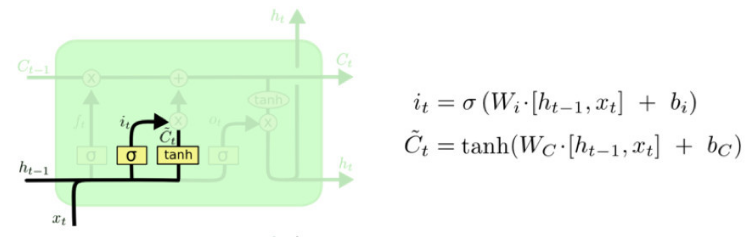
\includegraphics[scale=0.4]{t时刻的记忆计算过程}
\end{figure}

第三步:更新旧细胞状态的时间,$C_{t-1}$更新为$C_t$。
\begin{figure}[H]
	\centering
	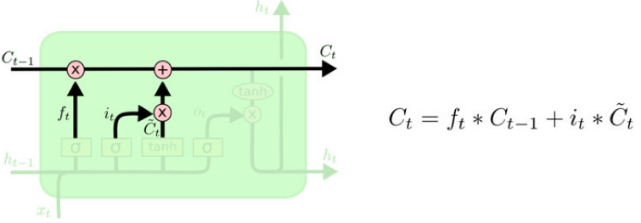
\includegraphics[scale=0.4]{更新时间}
\end{figure}

第四步:输出门,确定输出什么值。
\begin{figure}[H]
	\centering
	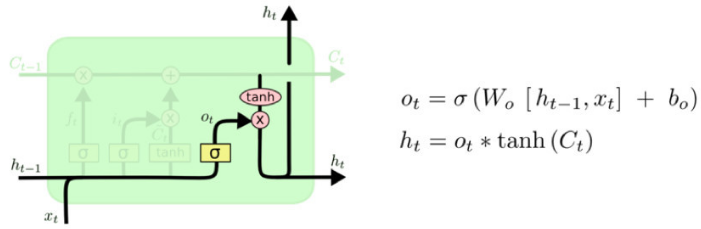
\includegraphics[scale=0.4]{确定输出值}
\end{figure}
\subsection{LSTM变体}
\begin{center}
	1.GRU
\end{center}

Gated Recurrent Unit.将遗忘门和输入门结合作为“更新门”(update gate)。序列中不同的位置的单词对当前隐藏层的状态的影响不同,每个前面状态对当前的影响进行距离加权,距离越远,权值越小。在产生error时,误差可能是由某一个或某几个单词引发,应当仅仅对单词weight进行更新。

GRU首先根据当前输入单词向量word vector在前一个隐藏层的状态中计算出update gate和reset gate。再根据reset gate,当前word vector以及前一个隐藏层计算新的记忆单元内容。

当reset gate为1的时候,前一个隐藏层计算新的记忆单元内容忽略之前的所有记忆单元内容,最终的记忆是之前的隐藏层与新的记忆单元内容的结合。

\begin{figure}[htbp]
	\centering
	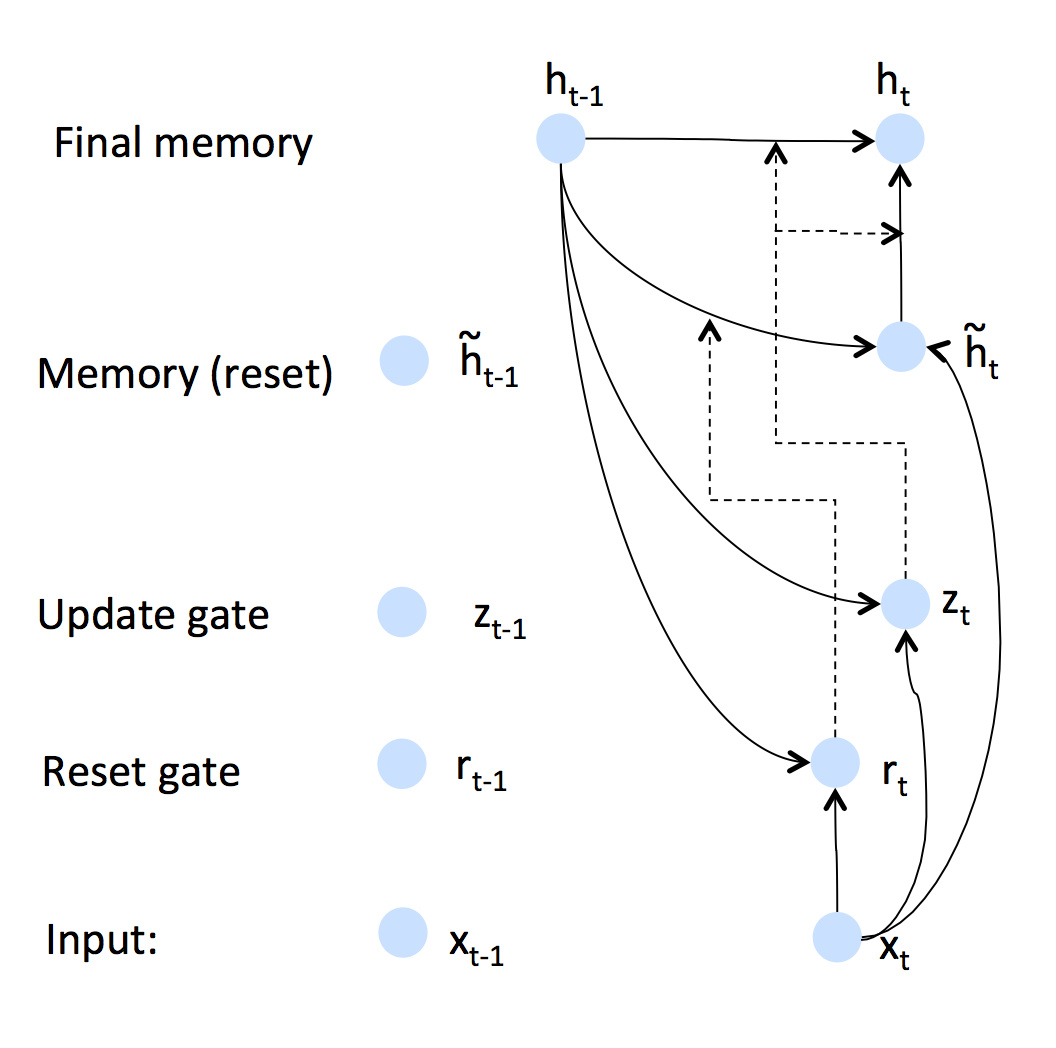
\includegraphics[scale=0.2]{GRU结构图}
\end{figure}
\begin{align*}
	z_t=\sigma(W^{(z)}x_t+U^{(z)}h_{t-1})	\\
	r_t=\sigma(W^{(r)}x_t+U^{(r)}h_{t-1})	\\
	\widetilde{h}_t = tanh(Wx_t + r_tUh_{t-1}) 	\\
	h_t=z_th_{t-1}+(1-z_t)\widetilde{h}_t
\end{align*}

\begin{center}
	2.CW-RNN
\end{center} 

一种使用时钟频率来驱动的RNN。它将隐藏层分为几组,每组按照自己规定的时钟频率对输入进行处理,将时钟时间进行离散化,然后在不同的时间点,不同的隐藏层组中工作,加快网络的训练。

CW-RNN包括输入层,隐藏层,输出层。输入层到隐藏层的连接,隐藏层到输出层的连接为前向连接。

\begin{figure}[htbp]
	\centering
	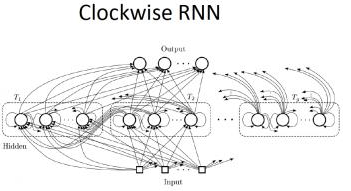
\includegraphics[scale=0.7]{CW-RNN结构图}
\end{figure}
\subsection{RNN的应用}
\begin{center}
	(1).机器翻译(Machine Transtation)
\end{center}

机器翻译是将一种源语言语句变成意思相同的另一种语言语句。与语言模型关键的区别在于:需要将源语言序列输入后,才能进行输出。

\begin{figure}[H]
	\centering
	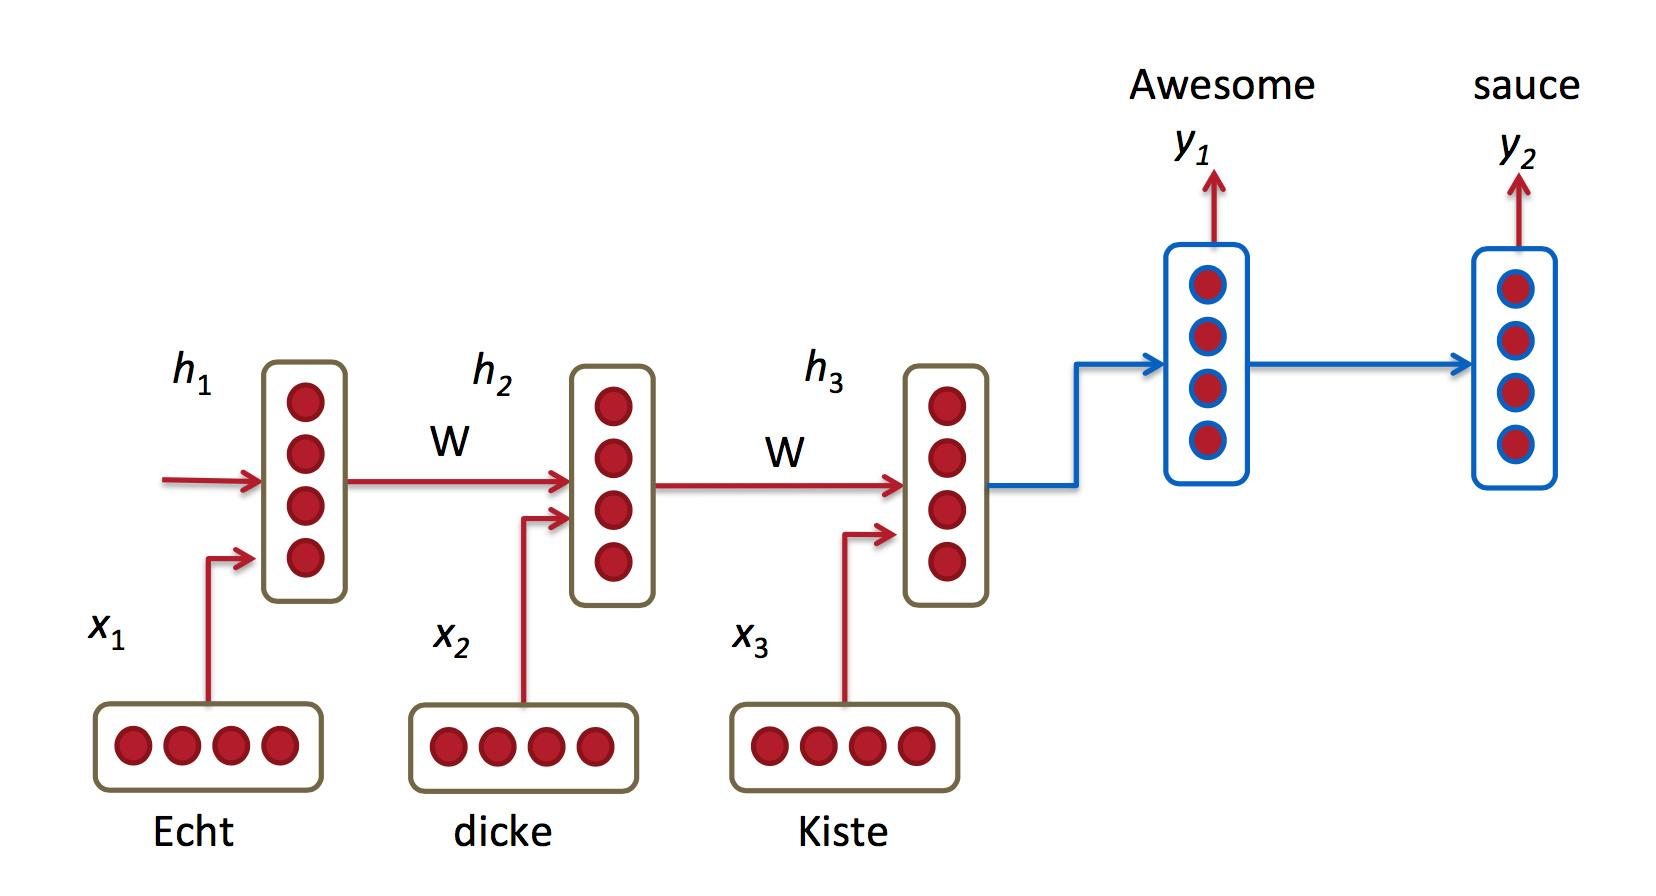
\includegraphics[scale=0.2]{机器翻译示例}
\end{figure}

\begin{center}
	(2)语言识别(Speech Recognition)
\end{center}

语音识别是指给一段声波的声音信号,预测该声波对应的某种指定源语音的语句以及该语句的概率值。

\begin{center}
	(3)图像描述生成(Generating Image Descriptions)
\end{center}

将CNN和RNN结合进行图像描述自动生成,该组合模型能够根据图像的特征生成描述。

\begin{figure}[H]
	\centering
	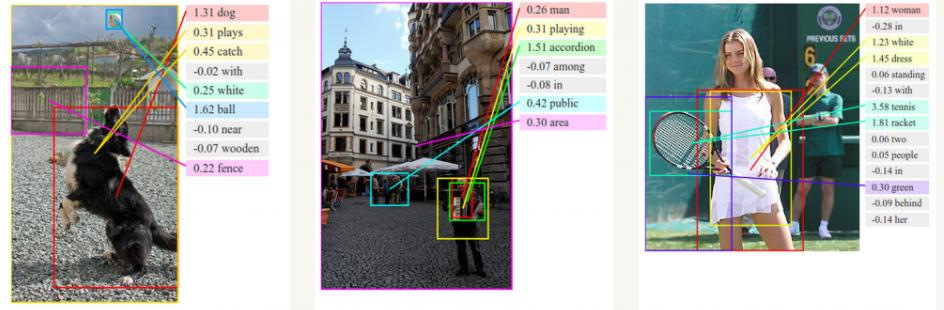
\includegraphics[scale=0.3]{CNN和RNN结合自动生成图片描述}
\end{figure}

\subsection{循环神经网络实现}
\subsubsection{RNN}
\begin{Python}{RNN案例}
	import torch
	import torch.nn as nn
	import torchvision.datasets as dsets
	import torchvision.transforms as transforms
	from torch.autograd import Variable
	
	# Hyper Parameters
	sequence_length = 28
	input_size = 28
	hidden_size = 128
	num_layers = 2
	num_classes = 10
	batch_size = 100
	num_epochs = 2
	learning_rate = 0.01
	
	# MNIST Dataset
	train_dataset = dsets.MNIST(root='./data/',
	train=True,
	transform=transforms.ToTensor(),
	download=True)
	
	test_dataset = dsets.MNIST(root='./data/',
	train=False,
	transform=transforms.ToTensor())
	
	# Data Loader (Input Pipeline)
	train_loader = torch.utils.data.DataLoader(dataset=train_dataset,
	batch_size=batch_size,
	shuffle=True)
	
	test_loader = torch.utils.data.DataLoader(dataset=test_dataset,
	batch_size=batch_size,
	shuffle=False)
	
	
	# RNN Model (Many-to-One)
	class RNN(nn.Module):
	def __init__(self, input_size, hidden_size, num_layers, num_classes):
	super(RNN, self).__init__()
	self.hidden_size = hidden_size
	self.num_layers = num_layers
	self.lstm = nn.LSTM(input_size, hidden_size, num_layers, batch_first=True)
	self.fc = nn.Linear(hidden_size, num_classes)
	
	def forward(self, x):
	# Set initial states
	h0 = Variable(torch.zeros(self.num_layers, x.size(0), self.hidden_size))
	c0 = Variable(torch.zeros(self.num_layers, x.size(0), self.hidden_size))
	
	# Forward propagate RNN
	out, _ = self.lstm(x, (h0, c0))
	
	# Decode hidden state of last time step
	out = self.fc(out[:, -1, :])
	return out
	
	
	rnn = RNN(input_size, hidden_size, num_layers, num_classes)
	
	# Loss and Optimizer
	criterion = nn.CrossEntropyLoss()
	optimizer = torch.optim.Adam(rnn.parameters(), lr=learning_rate)
	
	# Train the Model
	for epoch in range(num_epochs):
	for i, (images, labels) in enumerate(train_loader):
	images = Variable(images.view(-1, sequence_length, input_size))
	labels = Variable(labels)
	
	# Forward + Backward + Optimize
	optimizer.zero_grad()
	outputs = rnn(images)
	loss = criterion(outputs, labels)
	loss.backward()
	optimizer.step()
	
	if (i + 1) % 100 == 0:
	print('Epoch [%d/%d], Step [%d/%d], Loss: %.4f'
	% (epoch + 1, num_epochs, i + 1, len(train_dataset) // batch_size, loss))
	
	# Test the Model
	correct = 0
	total = 0
	for images, labels in test_loader:
	images = Variable(images.view(-1, sequence_length, input_size))
	outputs = rnn(images)
	_, predicted = torch.max(outputs.data, 1)
	total += labels.size(0)
	correct += (predicted.cpu() == labels).sum()
	
	print('Test Accuracy of the model on the 10000 test images: %d %%' % (100 * correct / total))
	
	# Save the Model
	torch.save(rnn.state_dict(), 'rnn.pkl')
	
	#Output:...
	#       Epoch [2/2], Step [400/600], Loss: 0.1151
	#       Epoch [2/2], Step [500/600], Loss: 0.0281
	#       Epoch [2/2], Step [600/600], Loss: 0.0728
	#       Test Accuracy of the model on the 10000 test images: 97 %
\end{Python}

\subsubsection{双向RNN}
\begin{Python}{双向RNN案例}
	import torch
	import torch.nn as nn
	import torchvision.datasets as dsets
	import torchvision.transforms as transforms
	from torch.autograd import Variable
	
	# Hyper Parameters
	sequence_length = 28
	input_size = 28
	hidden_size = 128
	num_layers = 2
	num_classes = 10
	batch_size = 100
	num_epochs = 2
	learning_rate = 0.003
	
	# MNIST Dataset
	train_dataset = dsets.MNIST(root='./data/',
	train=True,
	transform=transforms.ToTensor(),
	download=True)
	
	test_dataset = dsets.MNIST(root='./data/',
	train=False,
	transform=transforms.ToTensor())
	
	# Data Loader (Input Pipeline)
	train_loader = torch.utils.data.DataLoader(dataset=train_dataset,
	batch_size=batch_size,
	shuffle=True)
	
	test_loader = torch.utils.data.DataLoader(dataset=test_dataset,
	batch_size=batch_size,
	shuffle=False)
	
	
	# BiRNN Model (Many-to-One)
	class BiRNN(nn.Module):
	def __init__(self, input_size, hidden_size, num_layers, num_classes):
	super(BiRNN, self).__init__()
	self.hidden_size = hidden_size
	self.num_layers = num_layers
	self.lstm = nn.LSTM(input_size, hidden_size, num_layers,
	batch_first=True, bidirectional=True)
	self.fc = nn.Linear(hidden_size * 2, num_classes)  # 2 for bidirection
	
	def forward(self, x):
	# Set initial states
	h0 = Variable(torch.zeros(self.num_layers * 2, x.size(0), self.hidden_size))  # 2 for bidirection
	c0 = Variable(torch.zeros(self.num_layers * 2, x.size(0), self.hidden_size))
	
	# Forward propagate RNN
	out, _ = self.lstm(x, (h0, c0))
	
	# Decode hidden state of last time step
	out = self.fc(out[:, -1, :])
	return out
	
	
	rnn = BiRNN(input_size, hidden_size, num_layers, num_classes)
	
	# Loss and Optimizer
	criterion = nn.CrossEntropyLoss()
	optimizer = torch.optim.Adam(rnn.parameters(), lr=learning_rate)
	
	# Train the Model
	for epoch in range(num_epochs):
	for i, (images, labels) in enumerate(train_loader):
	images = Variable(images.view(-1, sequence_length, input_size))
	labels = Variable(labels)
	
	# Forward + Backward + Optimize
	optimizer.zero_grad()
	outputs = rnn(images)
	loss = criterion(outputs, labels)
	loss.backward()
	optimizer.step()
	
	if (i + 1) % 100 == 0:
	print('Epoch [%d/%d], Step [%d/%d], Loss: %.4f'
	% (epoch + 1, num_epochs, i + 1, len(train_dataset) // batch_size, loss))
	
	# Test the Model
	correct = 0
	total = 0
	for images, labels in test_loader:
	images = Variable(images.view(-1, sequence_length, input_size))
	outputs = rnn(images)
	_, predicted = torch.max(outputs.data, 1)
	total += labels.size(0)
	correct += (predicted.cpu() == labels).sum()
	
	print('Test Accuracy of the model on the 10000 test images: %d %%' % (100 * correct / total))
	
	# Save the Model
	torch.save(rnn.state_dict(), 'rnn.pkl')
	
	#Output:...
	#       Epoch [2/2], Step [300/600], Loss: 0.1400
	#       Epoch [2/2], Step [400/600], Loss: 0.0729
	#       Epoch [2/2], Step [500/600], Loss: 0.1303
	#       Epoch [2/2], Step [600/600], Loss: 0.0694
	#       Test Accuracy of the model on the 10000 test images: 98 %
\end{Python}	
\end{document}